\documentclass[12pt]{article}
\usepackage[utf8]{inputenc}
\usepackage[T1]{fontenc}
\usepackage{amsmath}
\usepackage{amsfonts}
\usepackage{amssymb}
\usepackage[version=4]{mhchem}
\usepackage{stmaryrd}
\usepackage{graphicx}
\usepackage[export]{adjustbox}

\usepackage{listings} % Required for insertion of code
\usepackage{xcolor} % Required for custom colors

% Define custom colors
\definecolor{codegreen}{rgb}{0,0.6,0}
\definecolor{codegray}{rgb}{0.5,0.5,0.5}
\definecolor{codepurple}{rgb}{0.58,0,0.82}
\definecolor{backcolour}{rgb}{0.95,0.95,0.92}

% Setup the style for code listings
\lstdefinestyle{mystyle}{
    backgroundcolor=\color{backcolour},   
    commentstyle=\color{codegreen},
    keywordstyle=\color{magenta},
    numberstyle=\tiny\color{codegray},
    stringstyle=\color{codepurple},
    basicstyle=\ttfamily\footnotesize,
    breakatwhitespace=false,         
    breaklines=true,                 
    captionpos=b,                    
    keepspaces=true,                 
    numbers=left,                    
    numbersep=5pt,                  
    showspaces=false,                
    showstringspaces=false,
    showtabs=false,                  
    tabsize=2
}

% Activate the style
\lstset{style=mystyle}

\graphicspath{ {./images/} }

\title{PROBLEMS: }

\author{}
\date{}


\begin{document}
\maketitle
\emph{I have an extension from the professor until 3/11}\\\\aaq q
READING: Section 19.6 in Shankar on two particle scattering.

Some facts that might come in handy:


\begin{align*}
j_{\ell}(x) & =\sqrt{\frac{\pi}{2 x}} J_{\ell+\frac{1}{2}}(x)  \tag{1}\\
n_{\ell}(x) & =\sqrt{\frac{\pi}{2 x}} Y_{\ell+\frac{1}{2}}(x)  \tag{2}\\
h_{\ell}^{(1)}(x) & =\sqrt{\frac{\pi}{2 x}} H_{\ell+\frac{1}{2}}^{(1)}(x)  \tag{3}\\
J_{\nu}(x) & \sim \sqrt{\frac{2}{\pi x}} \cos \left(x-\nu \frac{\pi}{2}-\frac{\pi}{4}\right)  \tag{4}\\
H_{\nu}^{(1)}(x) & \sim \sqrt{\frac{2}{\pi x}} e^{i\left(x-\nu \frac{\pi}{2}-\frac{\pi}{4}\right)} . \tag{5}
\end{align*}

\section{}
\begin{enumerate}
  \setcounter{enumi}{32}
  \item Show that the total cross section we computed in the partial wave expansion,
\end{enumerate}


\begin{equation*}
\sigma_{T}(p)=\frac{4 \pi}{p^{2}} \sum_{j=0}^{\infty}(2 j+1) \sin ^{2} \delta_{j}(p) \tag{6}
\end{equation*}


is in agreement with the optical theorem. That is, start with the optical theorem and derive the expression above.\\
The optical theorem is given as:
$$
\sigma_T(p)=\frac{4 \pi}{p} \Im f(p ; 1)
$$

The total cross section is equal to $4 \pi / p$ times the imaginary part of the forward scattering amplitude. So we want to find that $\frac{1}{p} \Im f(p ; 1)= \sum_{j=0}^{\infty}(2 j+1) \sin ^{2} \delta_{j}(p)$. First, we start by evaluating $f(p ; 1)$. The partial with expansion for the scattering amplitude is given by:
\begin{equation}
f(\mathbf{p}, \mathbf{q})=f(p ; \cos \theta)=\frac{1}{2 i p} \sum_{j=0}^{\infty}(2 j+1)\left[e^{2 i \delta_j(p)}-1\right] P_j(\cos \theta)
\end{equation}
The Legendre polynomials are normalized, so $P_{j}(1)=1 \forall j$. Therefore, we can write the forward scattering amplitude as:
\begin{equation}
f(p ; 1)=\frac{1}{2 i p} \sum_{j=0}^{\infty}(2 j+1)\left[e^{2 i \delta_j(p)}-1\right]
\end{equation}
We can rewrite the exponential piece using elders formula as:
\begin{equation}
e^{2 i \delta_j(p)}-1=\cos (2 \delta_j(p))+i \sin (2 \delta_j(p))-1
\end{equation}
Now, we can use the identity that $\cos(2\delta _{j}(p))-1=-2\sin^{2}(\delta_{j}(p))$ and also the double angle identity for $\sin(2\delta_{j}(p))= 2\sin(\delta_{j}(p))\cos(\delta_{j}(p))$. Therefore, we can write the forward scattering amplitude as:
\begin{equation}
f(p ; 1)=\frac{1}{2 i p} \sum_{j=0}^{\infty}(2 j+1)\left[-2\sin^{2}(\delta_{j}(p))+2i\sin(\delta_{j}(p))\cos(\delta_{j}(p))\right]
\end{equation}
We now recognize that the real part inside the summation will become the imaginary part of the scattering in pluto because of the inverse dependence on $i$. Therefore, we can write the imaginary part of the scattering amplitude as:
\begin{equation}
\Im f(p ; 1)=\frac{1}{ p} \sum_{j=0}^{\infty}(2 j+1) \sin ^{2} \delta_{j}(p)
\end{equation}
Plugging this into the optical theorem, we get:
\begin{equation}
\sigma_T(p)=\frac{4 \pi}{p} \Im f(p ; 1)=\frac{4 \pi}{p^{2}} \sum_{j=0}^{\infty}(2 j+1) \sin ^{2} \delta_{j}(p)
\end{equation}
\section{}
\begin{enumerate}
  \setcounter{enumi}{33}
  \item We have discussed the "central force problem". Consider a particle of mass $m$ under the influence of the following potential:
\end{enumerate}

\[
V(r)= \begin{cases}V_{0}, & 0 \leq r \leq a  \tag{7}\\ 0, & a<r\end{cases}
\]

where $V_{0}$ is a constant.
\subsection{}
(a) If $V_{0}<0$, what can you say about the phase shift, $\delta_{\ell}$, in partial wave $\ell$, for scattering on this potential. What if $V_{0}>0$ ? For $V_{0} \neq 0$ is it possible for the scattering amplitude in a given partial wave to vanish?\\\\
For an attractive potential, lakes $V_{0}<0$, the phase shift will be positive. This is because the scattered particle will oscillate more frequently near the potential and incur a phase shift with respect to a unscattered particle. For a repulsive potential, like $V_{0}>0$, the phase shift will be negative. This is because the particle will oscillate less frequently near the repulsive potential and incur a negative phase shift with respect to a unscattered particle. That scattering amplitude in the partial wave expansion is given by:
\begin{equation}
f(\mathbf{p}, \mathbf{q})=f(p ; \cos \theta)=\frac{1}{2 i p} \sum_{j=0}^{\infty}(2 j+1)\left[e^{2 i \delta_j(p)}-1\right] P_j(\cos \theta)
\end{equation}
This could only vanish if we have:
\begin{equation}
e^{2 i \delta_j(p)}=1 \rightarrow \delta_j(p)=n\pi
\end{equation}
where $n$ is an integer. So the answer is that the scattering and fluted can sometimes vanish when the partial wave face shift satisfies the given quantization condition.
\subsection{}
(b) Write down the Schrödinger equation for the wave function $\psi(\mathbf{x})$. Consider solutions which are simultaneous eigenvectors of $H, \mathbf{L}^{2}$, and $L_{z}$. Solve the angular dependence, and reduce the remaining problem to a problem in one variable.
The Schrödinger equation for this spherically symmetric potential is given by:
\begin{equation}
\left[-\frac{\hbar^{2}}{2 m} \nabla^{2}+V(r)\right] \psi(\mathbf{x})=E \psi(\mathbf{x})
\end{equation}
Because this is a spherically symmetric problem, we can express the Laplacian in spherical coordinates as:
\begin{equation}
\nabla^{2}=\frac{1}{r^{2}} \frac{\partial}{\partial r}\left(r^{2} \frac{\partial}{\partial r}\right)-\frac{\mathbf{L}^{2}}{\hbar^{2} r^{2}}
\end{equation}
We employ the method of separation of variables to guess a solution of the form:
\begin{equation}
\psi(\mathbf{x})=R(r)Y_{\ell m}(\theta, \phi)
\end{equation}
For the radial solution of the wave function, we have the differential equation:
\begin{equation}
\chi_{\ell}^{\prime \prime}+\left[k^2-\frac{\ell(\ell+1)}{r^2}-2 m V(r)\right] \chi_{\ell}=0
\end{equation}
where $k^2=2 m E / \hbar^2$ and $\chi_{\ell}=r R_{\ell}$. 
We know that the solution of this radial. eqn inside the potential is given by:
\begin{equation}
\psi=\sum_{\ell=0}^{\infty}(i)^{\ell}(2 \ell+1) R_{\ell}(k ; r) P_{\ell}(\cos \theta)
\end{equation}
The solution given in the notes is given by:
\begin{equation}
\psi(\mathbf{x})=\sum_{\ell=0}^{\infty} \sum_{m=-\ell}^{\ell}\left[A_{\ell m} j_{\ell}(k r)+B_{\ell m} n_{\ell}(k r)\right] P_l^m(\theta) e^{i m \phi}
\end{equation}
But then the second coefficient is 0 because $n_{\ell}(k r)$ is not tegular near the origin, so we just simplify the solution to:
\begin{equation}
\psi(\mathbf{x})=\sum_{\ell=0}^{\infty} \sum_{m=-\ell}^{\ell}A_{\ell m} j_{\ell}(k r) P_l^m(\theta) e^{i m \phi}
\end{equation}
and the solution outside the potential is given by:
\begin{equation}
\psi=\sum_{\ell=0}^{\infty}(i)^{\ell}(2 \ell+1)\left[j_{\ell}(k r)+\frac{1}{2} \alpha_{\ell} h_{\ell}^{(1)}(k r)\right] P_{\ell}(\cos \theta)
\end{equation}
Now, we have to match the solution in on both sides of the potential. So the limit of the wfn as it approches $a$ from the left must equal the limit of the wfn as it approaches $a$ from the right.
\begin{equation}
\lim _{r \rightarrow a^-} \psi_{\text {inside }}=\lim _{r \rightarrow a^+} \psi_{\text {outside }}
\end{equation}
Likewise the derivative of the wfn as it approaches $a$ from the left must equal the derivative of the wfn as it approaches $a$ from the right.
\begin{equation}
\lim _{r \rightarrow a^-} \frac{d \psi_{\text {inside }}}{d r}=\lim _{r \rightarrow a^+} \frac{d \psi_{\text {outside }}}{d r}
\end{equation}
defining $\psi_{\text {inside }}$ and $\psi_{\text {outside }}$ as the wfn inside and outside of the potential:
\begin{equation}
\psi_{\text {inside }}=\sum_{\ell=0}^{\infty} \sum_{m=-\ell}^{\ell}A_{\ell m} j_{\ell}(k r) P_l^m(\theta) e^{i m \phi}
\end{equation}
\begin{equation}
\psi_{\text {outside }}=\sum_{\ell=0}^{\infty}(i)^{\ell}(2 \ell+1)\left[j_{\ell}(k r)+\frac{1}{2} \alpha_{\ell} h_{\ell}^{(1)}(k r)\right] P_{\ell}(\cos \theta)
\end{equation}
First, we impose the first equality:
\begin{equation}
\sum_{\ell=0}^{\infty} \sum_{m=-\ell}^{\ell}A_{\ell m} j_{\ell}(k a) P_l^m(\theta) e^{i m \phi}= \sum_{\ell=0}^{\infty}(i)^{\ell}(2 \ell+1)\left[j_{\ell}(k a)+\frac{1}{2} \alpha_{\ell} h_{\ell}^{(1)}(k a)\right] P_{\ell}(\cos \theta)
\end{equation}
We can get rid of the sum on both sides over $\ell$:
\begin{equation}
\sum_{m=-\ell}^{\ell}A_{\ell m} j_{\ell}(k a) P_l^m(\theta) e^{i m \phi}= (i)^{\ell}(2 \ell+1)\left[j_{\ell}(k a)+\frac{1}{2} \alpha_{\ell} h_{\ell}^{(1)}(k a)\right] P_{\ell}(\cos \theta)
\end{equation}
Since the scattering is along the z-axis, we can set $m=0$ and so $e^{i m \phi}=1$. We also know that the associated Legendre polymial at $m=0$ is just $P_{\ell}(\cos \theta)$. Then, by the orthogonality of the Legendre polynomials, we can get rid of the sum over $m$:
\begin{equation}
A_{\ell 0} j_{\ell}(k a)= (i)^{\ell}(2 \ell+1)\left[j_{\ell}(k a)+\frac{1}{2} \alpha_{\ell} h_{\ell}^{(1)}(k a)\right]
\end{equation}
Now we impose the second equality:
\begin{equation}
\sum_{\ell=0}^{\infty} \sum_{m=-\ell}^{\ell}A_{\ell m} j_{\ell}^{\prime}(k a) P_l^m(\theta) e^{i m \phi}= \sum_{\ell=0}^{\infty}(i)^{\ell}(2 \ell+1)\left[j_{\ell}^{\prime}(k a)+\frac{1}{2} \alpha_{\ell} h_{\ell}^{(1) \prime}(k a)\right] P_{\ell}(\cos \theta)
\end{equation}
Using the same logic as before, we can get rid of the sum over $m$ and set $m=0$ and $e^{i m \phi}=1$. Then, by the orthogonality of the Legendre polynomials, we can get rid of the sum over $m$:
\begin{equation}
A_{\ell 0} j_{\ell}^{\prime}(k a)= (i)^{\ell}(2 \ell+1)\left[j_{\ell}^{\prime}(k a)+\frac{1}{2} \alpha_{\ell} h_{\ell}^{(1) \prime}(k a)\right]
\end{equation}
Now, we divide the first equality for $A_{\ell 0}$ by the second equality for $A_{\ell 0}$, which simply gives a relation purely in terms of $\alpha_{\ell}$:
\begin{equation}
\frac{j_{\ell}(k a)}{j_{\ell}^{\prime}(k a)}= \frac{(i)^{\ell}(2 \ell+1)\left[j_{\ell}(k a)+\frac{1}{2} \alpha_{\ell} h_{\ell}^{(1)}(k a)\right]}{(i)^{\ell}(2 \ell+1)\left[j_{\ell}^{\prime}(k a)+\frac{1}{2} \alpha_{\ell} h_{\ell}^{(1) \prime}(k a)\right]}
\end{equation}
We cancel out the $(i)^{\ell}(2 \ell+1)$ terms:
\begin{equation}
\frac{j_{\ell}(k a)}{j_{\ell}^{\prime}(k a)}= \frac{j_{\ell}(k a)+\frac{1}{2} \alpha_{\ell} h_{\ell}^{(1)}(k a)}{j_{\ell}^{\prime}(k a)+\frac{1}{2} \alpha_{\ell} h_{\ell}^{(1) \prime}(k a)}
\end{equation}
We can solve for $\alpha_{\ell}$:
\begin{equation}
\alpha_{\ell}=-2 \frac{j_{\ell}(k a)}{h_{\ell}^{(1)}(k a)} \frac{j_{\ell}^{\prime}(k a)}{j_{\ell}(k a)-j_{\ell}^{\prime}(k a)}
\end{equation}
\subsection{}
(c) Let $E>0$ be an eigenvalue of the Hamiltonian, $H$. Solve the Schrödinger equation for eigenstates $\psi(\mathbf{x})$. It will probably be convenient to use the quantity $K=\sqrt{2 m\left(V_{0}-E\right)}$.

You may wish to express your solution for the phase shifts $\alpha_{\ell}$ in terms of the "logarithmic derivative".


\begin{equation*}
\left.L_{\ell} \equiv \frac{d \log j_{\ell}(i K r)}{d \log r}\right|_{x=a} \tag{8}
\end{equation*}


Hint: You will probably benefit by thinking about solutions in the form of spherical Bessel/Neumann functions, and/or spherical Hankel functions. See, e.g., section 12.6 of Shankar.
\subsection{}

(d) Consider the limit as $r \rightarrow \infty$ for your solutions, and give an interpretation in terms of spherical waves.
\section{}
\begin{enumerate}
  \setcounter{enumi}{34}
  \item Consider scattering from the simple potential:
\end{enumerate}

$$
V(\mathbf{x})= \begin{cases}V_{0} & r=|\mathbf{x}|<R \\ 0 & r>R\end{cases}
$$

In the low energy limit, we might only look at $S$-wave $\ell=0$ scattering. However, in the high energy limit, we expect scattering in other partial waves to become significant. For simplicity, let us here consider scattering on a hard sphere, $V_{0} \rightarrow \infty$.
\subsection{}
(a) For a hard sphere potential, calculate the total cross section in partial wave $\ell$. Give the exact result, i.e., don't take the high energy limit yet. You may quote your answer in terms of the spherical Bessel functions.\\\\
And expression for the total cross section is:
\begin{equation}
\sigma_T=\int_{(4 \pi)} d \Omega|f(k ; \theta)|^2
\end{equation}
The scattering amplitude is given by:
\begin{equation}
f(k ; \theta)=\frac{1}{2 i k} \sum_{\ell=0}^{\infty}(2 \ell+1)\left(e^{2 i \delta_{\ell}}-1\right) P_{\ell}(\cos \theta) .
\end{equation}
where we know that the phase shift is given by:
\begin{equation}
\alpha_{\ell}=e^{2 i \delta_{\ell}}-1
\end{equation}
We want to compute the phase shift in terms of the spherical vessel functions . we also need to consider that the potential inside of the sphere will be infinite, so this suggests the boundary condition of the wfn being 0 at $r=R$.
The wave function outside of the sphere is given by:\\
Outside the sphere $r=R$ we may write:
$$
\psi=\sum_{\ell=0}^{\infty}(i)^{\ell}(2 \ell+1)\left[j_{\ell}(k r)+\frac{1}{2} \alpha_{\ell} h_{\ell}^{(1)}(k r)\right] P_{\ell}(\cos \theta),
$$
where $h_{\ell}^{(1)}$ is the spherical Hankel function of the first kind:
$$
\begin{aligned}
h_{\ell}^{(1)}(k r) & =j_{\ell}(k r)+i n_{\ell}(k r) \\
\rightarrow_{k r \rightarrow \infty} & \frac{1}{(i)^{\ell+1}} \frac{e^{i k r}}{k r} .
\end{aligned}
$$
We require that $\psi (r=R)=0$, so we have:
\begin{equation}
\sum_{\ell=0}^{\infty}(i)^{\ell}(2 \ell+1)\left[j_{\ell}(k R)+\frac{1}{2} \alpha_{\ell} h_{\ell}^{(1)}(k R)\right] P_{\ell}(\cos \theta)=0
\end{equation}
All of the powerful waves are independent, so the inside of the summation must equal to 0.
\begin{equation}
j_{\ell}(k R)+\frac{1}{2} \alpha_{\ell} h_{\ell}^{(1)}(k R)=0
\end{equation}
We can solve for $\alpha_{\ell}$ and we know it must equal $e^{2 i \delta_{\ell}}-1$.
\begin{equation}
\alpha_{\ell}=-2 \frac{j_{\ell}(k R)}{h_{\ell}^{(1)}(k R)} = e^{2 i \delta_{\ell}}-1
\end{equation}
We know that an expression for the total cross section for a given angular momentum state is given by:
\begin{equation}
  \sigma _{T \ell} = \frac{4 \pi}{k^2} (2 \ell + 1) \sin^2 \delta_{\ell}
\end{equation}
Now we want to see with the exponential expansion for the square of the sign is:
\begin{equation}
\sin^2 \delta_{\ell} = \left| \frac{e^{i \delta_{\ell}}-e^{- i \delta_{\ell}}}{2i} \right|^2
\end{equation}
We can factor out a $e^{-i \delta_{\ell}}$ within the parentheses:
\begin{equation}
\sin^2 \delta_{\ell} = \left| e^{-i \delta_{\ell}} \frac{e^{2i \delta_{\ell}}-1}{2i} \right|^2
\end{equation}
The $\frac{e^-i \delta_{\ell}}{i}$ will vanish when we take the absolute value and square it. Therefore, we simpifly the expression to:
\begin{equation}
\sin^2 \delta_{\ell} = \left| \frac{e^{2i \delta_{\ell}}-1}{2} \right|^2
\end{equation}
But we know that $\alpha_{\ell}=e^{2 i \delta_{\ell}}-1$, so we can write this as:
\begin{equation}
\sin^2 \delta_{\ell} = \left| \frac{\alpha_{\ell}}{2} \right|^2
\end{equation}
So the total cross section is given by:
\begin{equation}
\sigma _{T \ell} = \frac{4 \pi}{k^2} (2 \ell + 1) \left| \frac{\alpha_{\ell}}{2} \right|^2
\end{equation}
where $\alpha_{\ell}$ is given by:
\begin{equation}
\alpha_{\ell}=-2 \frac{j_{\ell}(k R)}{h_{\ell}^{(1)}(k R)}
\end{equation}
\subsection{}
(b) Find a simple expression for the phase shift $\delta_{\ell}$ in the high energy limit $(k R \gg$ $\ell$ ). Keep terms up to $\mathrm{O}(1)$ in your result.\\\\
We know that we have the equality:
\begin{equation}
\alpha_{\ell}=-2 \frac{j_{\ell}(k R)}{h_{\ell}^{(1)}(k R)} = e^{2 i \delta_{\ell}}-1
\end{equation}
Isolation the exponential term and then taking the natural logarithm of both sides, we get:
\begin{equation}
2 i \delta_{\ell} = \ln \left( -2 \frac{j_{\ell}(k R)}{h_{\ell}^{(1)}(k R)} + 1 \right)
\end{equation}
Now, we are interested in interesting the behavior of the fraction in this high energy limit. We know that the form for the denominator is:
\begin{equation}
h_{\ell}^{(1)}(x) \sim \sqrt{\frac{2}{\pi x}} e^{i\left(x-(\ell+\frac{1}{2}) \frac{\pi}{2}-\frac{\pi}{4}\right)}
\end{equation}
And the form for the numerator is:
\begin{equation}
j_{\ell}(x) \sim \sqrt{\frac{2}{\pi x}} \cos \left(x-(\ell + \frac{1}{2})\frac{\pi }{2}-\frac{\pi}{4}\right)
\end{equation}
So we can write the fraction as:
\begin{equation}
-2 \frac{j_{\ell}(k R)}{h_{\ell}^{(1)}(k R)} \sim -2 \frac{\cos \left(k R-(\ell + \frac{1}{2})\frac{\pi }{2}-\frac{\pi}{4}\right)}{e^{i\left(k R-(\ell + \frac{1}{2})\frac{\pi }{2}-\frac{\pi}{4}\right)}}
\end{equation}
Now we recognize that $\cos(\theta ) = \frac{e^{i\theta}+e^{-i\theta}}{2}$, where here we have $\theta = k R-(\ell + \frac{1}{2})\frac{\pi }{2}-\frac{\pi}{4}$. So we can write the fraction as:
\begin{equation}
-2 \frac{j_{\ell}(k R)}{h_{\ell}^{(1)}(k R)} \sim -2 \frac{e^{i\left(k R-(\ell + \frac{1}{2})\frac{\pi }{2}-\frac{\pi}{4}\right)}+e^{-i\left(k R-(\ell + \frac{1}{2})\frac{\pi }{2}-\frac{\pi}{4}\right)}}{2e^{i\left(k R-(\ell + \frac{1}{2})\frac{\pi }{2}-\frac{\pi}{4}\right)}}
\end{equation}
Simplifying the fraction, we get:
\begin{equation}
-2 \frac{j_{\ell}(k R)}{h_{\ell}^{(1)}(k R)} \sim -1 + e^{-2i\left(k R-(\ell + \frac{1}{2})\frac{\pi }{2}-\frac{\pi}{4}\right)}
\end{equation}
This has to be equal to:
\begin{equation}
-2 \frac{j_{\ell}(k R)}{h_{\ell}^{(1)}(k R)} = -1 + e^{-2i\left(k R-(\ell + \frac{1}{2})\frac{\pi }{2}-\frac{\pi}{4}\right)} = e^{2 i \delta_{\ell}}-1
\end{equation}
So we can write the phase shift as:
\begin{equation}
\delta_{\ell} = -k R+(\ell + \frac{1}{2})\frac{\pi }{2}+\frac{\pi}{4}
\end{equation}

\subsection{}
(c) Determine the total cross section (including all partial waves) in the high energy limit, $k R \rightarrow \infty$. [This is the only somewhat tricky part of this problem to calculate. One approach is as follows: Write down the total cross section in terms of your results for part (a). Then, for fixed $k$, consider which values of $\ell$ may be important in the sum. Neglect the other values of $\ell$, and make the high energy approximation to your part (a) result. Finally, evaluate the sum, either directly, or by turning it into an appropriate integral.]\\\\
This time we want to consider the total class section for all partial waves, so that expression becomes:
\begin{equation}
\sigma_T(p)=\frac{4 \pi}{p^2} \sum_{l=0}^{
\infty } (2 l+1) \sin ^2 \delta_l(p)
\end{equation}
We know that the phase shift is given by:
\begin{equation}
\delta_{\ell} = -k R+\ell \frac{\pi}{2}+\frac{\pi}{4} =\frac{\pi}{2} (\ell+1/2)-k R
\end{equation}
In the limit of large $kR$ whenever $kR \propto \ell$, the phase shift will be small. Because $\sin^2(\delta_{\ell})$ tense to 0, whenever $\delta_{\ell}$ is small, we can rewrite the upper bound in the summation for the total cast section:
\begin{equation}
\sigma_T(p)=\frac{4 \pi}{p^2} \sum_{l=0}^{kR} (2 l+1) \sin ^2 \delta_l(p)
\end{equation}
We can proceed by considering the average value that $\sin^2(\delta_{\ell})$ takes on in this summation up to $kR$:
\begin{equation}
\langle \sin^2(\delta_{\ell}) \rangle = \frac{1}{2} \left( \sin^2(\delta_{\ell}) + \sin^2(\delta_{\ell+1}) \right)
\end{equation}
where we consider both the even and odd values of $\ell$. Since $\delta_{\ell} = \frac{\pi}{2}\ell - kR + \frac{\pi}{4}$, then $\delta_{\ell+1} = \frac{\pi}{2}(\ell+1) - kR + \frac{\pi}{4} = \delta_{\ell} + \frac{\pi}{2}$. And since we know $\sin{(\delta_{\ell} + \frac{\pi}{2})} = \cos{(\delta_{\ell})}$, then $\sin^2(\delta_{\ell+1}) = \cos^2(\delta_{\ell})$. So we can write the average value of $\sin^2(\delta_{\ell})$ as:
\begin{equation}
\langle \sin^2(\delta_{\ell}) \rangle = \frac{1}{2} \left( \sin^2(\delta_{\ell}) + \cos^2(\delta_{\ell}) \right) = \frac{1}{2}
\end{equation}
So the total cross section is given by:
\begin{equation}
\sigma_T(p) = \frac{4 \pi}{p^2} \sum_{l=0}^{kR} (2 l+1) \frac{1}{2} = \frac{2 \pi}{p^2} \sum_{l=0}^{kR} (2 l+1)
\end{equation}
This is an arithmetic series, given by:
\begin{equation}
  \sigma_T(p) = \frac{2\pi (kR+1)^2}{p^2}
\end{equation}
% Inline Python code in the document
\begin{lstlisting}[language=Python]
from sympy import symbols, pi

# Define symbols
kR = symbols('kR')
p = symbols('p')

# Number of terms in the series
n = kR + 1

# Sum of the series
sum_series = n*(2*1 + (n-1)*2)/2

# Expression for sigma_T(p)
sigma_T_p = (2 * pi / p**2) * sum_series
sigma_T_p.simplify()
\end{lstlisting}
but then we know that $p \approx k$, so we can write the total cross section as:
\begin{equation}
\sigma_T(p) = \frac{2\pi (kR+1)^2}{k^2} \approx \frac{2\pi (kR)^2}{k^2} = 2\pi R^2
\end{equation}
% Now we can use the fact that $\sin^2(\delta_{\ell})= \sin^2(\frac{\pi}{4} (2\ell+1)-k R)$. Given that $\sin (\frac{\pi }{4} (2\ell+1)-k R) = \sin (\frac{\pi }{4} (2\ell+1)) \sin (kR) - \cos (\frac{\pi }{4} (2\ell+1)) \cos (kR)$, we can write $\sin^2(\delta_{\ell})$ as:
% \begin{equation}
% \sin^2(\delta_{\ell})= \left[ \sin (\frac{\pi }{4} (2\ell+1)) \sin (kR) - \cos (\frac{\pi }{4} (2\ell+1)) \cos (kR) \right]^2
% \end{equation}
% Notice that when $\ell$ is even
\section{}
\begin{enumerate}
  \setcounter{enumi}{35}
  \item Consider the graph in Fig. 1. The numbers from which this graph was made are available in the file Delta++PhaseShifts.txt in the module for week 9.
\end{enumerate}

Assume that the other phase shifts are negligible (e.g., "low energy" is reasonably accurate). The pion mass and energy here are sufficiently small that we can at least entertain the approximation of an infinitely heavy proton at rest - we'll assume this to be the case, in any event. Note that $T_{\pi}$ is the relativistic kinetic energy of the $\pi^{+}: T_{\pi}=\sqrt{P_{\pi}^{2}+m_{\pi}^{2}}-m_{\pi}$.
\subsection{}
(a) Is the $\pi^{+} p$ force principally attractive or repulsive (as shown in this figure)?\\\\
Attractive, because the face shifts are positive.
\subsection{}
(b) Plot the total cross section in mb (millibarns) as a function of energy, from $T_{\pi}=40$ to $200 \mathrm{MeV}$.\\\\
The total cross section is given by:
\begin{equation}
\sigma_T(p)=\frac{4 \pi}{p^2} \sum_j(2 j+1) \sin ^2 \delta_j(p)
\end{equation}
We can find the momentum of the pion using the formula:
\begin{equation}
T_{\pi}=\sqrt{P_{\pi}^{2}+m_{\pi}^{2}}-m_{\pi} \rightarrow P_{\pi}=\sqrt{T_{\pi}^{2}+2m_{\pi}T_{\pi}}
\end{equation}
And then we are only given the phase shifts for $j=0$ and $j=1$, So the total cross section is just a sum for these two partial waves. 
\begin{figure}
  \centering
  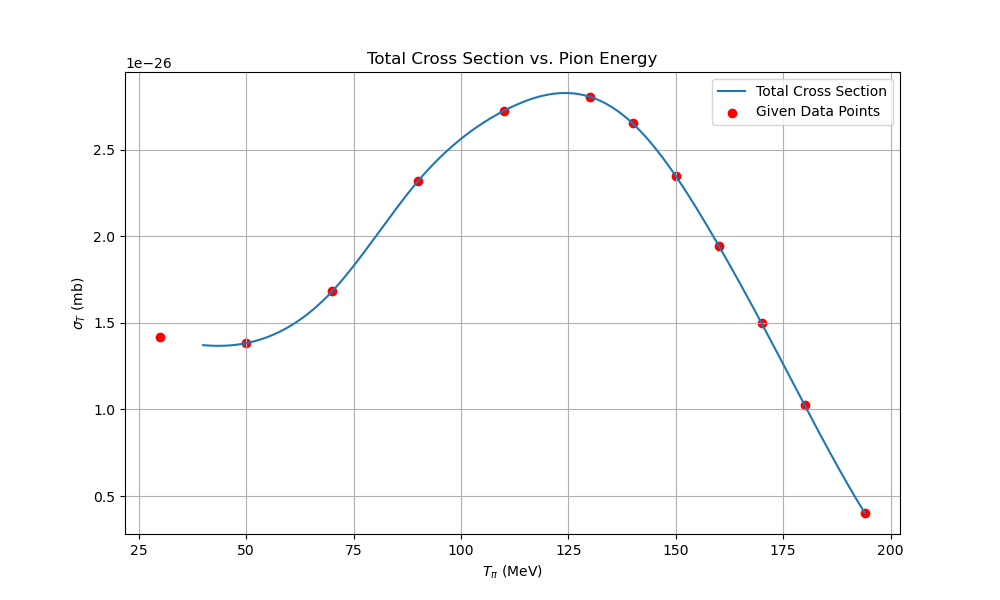
\includegraphics[max width=\textwidth]{total_cross_section.png}
\end{figure}
% Inline Python code in the document
% Inline Python code in the document
\begin{lstlisting}[language=Python]
import numpy as np
import scipy.constants as const
import matplotlib.pyplot as plt
from scipy.interpolate import interp1d

# Constants
m_pi = 139.6  # MeV/c^2
conversion_factor_to_mb = 10**31 / (const.hbar * const.c * 1e3)**2  # Convert to mb using hbar in MeV*s and c in m/s, then to m^2

# Given data
T_pi = np.array([30, 50, 70, 90, 110, 130, 140, 150, 160, 170, 180, 194])  # MeV
delta_0_deg = np.array([25]*len(T_pi))  # degrees, constant for all given T_pi
delta_1_deg = np.array([10, 18, 28, 43, 59, 78, 90, 100, 111, 122, 134, 154])  # degrees

# Convert degrees to radians
delta_0 = np.deg2rad(delta_0_deg)
delta_1 = np.deg2rad(delta_1_deg)

# Calculate momentum P_pi using the relativistic energy-momentum relation
P_pi = np.sqrt(T_pi**2 + 2*m_pi*T_pi)  # MeV/c

hbar_c_MeV_fm = 197.3269788  # hbar*c in MeV*fm
conversion_factor_to_mb = 10**-27  # 1 fm^2 = 10^-30 m^2, and 1 mb = 10^-31 m^2, so 1 fm^2 = 10 mb

# Adjusting the sigma_T calculation to use the correct conversion factor
def sigma_T_corrected(P_pi, delta_0, delta_1):
    return (4 * np.pi / (P_pi / hbar_c_MeV_fm)**2) * ((2*0+1) * np.sin(delta_0)**2 + (2*1+1) * np.sin(delta_1)**2) * conversion_factor_to_mb

# Recompute sigma_T with the corrected conversion
sigma_T_values = sigma_T_corrected(P_pi, delta_0, delta_1)


# Adjusting T_pi_plot to be within the given data range
T_pi_plot = np.linspace(40, 194, 400)
sigma_T_interp = interp1d(T_pi, sigma_T_values, kind='cubic', fill_value="extrapolate")

# Re-plotting with the adjusted range
plt.figure(figsize=(10, 6))
plt.plot(T_pi_plot, sigma_T_interp(T_pi_plot), label='Total Cross Section')
plt.scatter(T_pi, sigma_T_values, color='red', label='Given Data Points')  # Highlight the given data points

plt.title('Total Cross Section vs. Pion Energy')
plt.xlabel('$T_{\pi}$ (MeV)')
plt.ylabel('$\sigma_T$ (mb)')
plt.legend()
plt.grid(True)
plt.savefig('total_cross_section.png')


\end{lstlisting}

\subsection{}
(c) Plot the angular distribution of the scattered $\pi^{+}$at energies of 120, 140 and $160 \mathrm{MeV}$.\\\\
We know that the formula for the scattering amplitude is:
\begin{equation}
f(\mathbf{p}, \mathbf{q})=f(p ; \cos \theta)=\frac{1}{2 i p} \sum_{j=0}^{\infty}(2 j+1)\left[e^{2 i \delta_j(p)}-1\right] P_j(\cos \theta)
\end{equation}
Because we have a spin less particle, the total engler momentum has no contribution from the spin angular momentum, so we can substitute $j$ with $\ell$ everywhere:
\begin{equation}
f(\mathbf{p}, \mathbf{q})=f(p ; \cos \theta)=\frac{1}{2 i p} \sum_{\ell=0}^{\infty}(2 \ell+1)\left[e^{2 i \delta_{\ell}(p)}-1\right] P_{\ell}(\cos \theta)
\end{equation}
We know that the these shifts are negligible for $\ell > 1$, so we can just consider the first two partial waves in the sum:
\begin{equation}
f(p ; \cos \theta)=\frac{1}{2 i p} \left[(2 \cdot 0+1)\left(e^{2 i \delta_{0}(p)}-1\right) P_{0}(\cos \theta) + (2 \cdot 1+1)\left(e^{2 i \delta_{1}(p)}-1\right) P_{1}(\cos \theta)\right]
\end{equation}
where the first two Legendre polynomials are given by:
\begin{equation}
P_0(\cos \theta) = 1
\end{equation}
\begin{equation}
P_1(\cos \theta) = \cos \theta
\end{equation}
So the scattering amplitude is given by:
\begin{equation}
f(p ; \cos \theta)=\frac{1}{2 i p} \left[\left(e^{2 i \delta_{0}(p)}-1\right) + 3\left(e^{2 i \delta_{1}(p)}-1\right) \cos \theta\right]
\end{equation}
I performed a rough learner fit for the ps1 of 120 MeV, as it was not given.

The angler discretion is just the absolute value squared of this scattering amplitude:
\begin{equation}
|f(p ; \cos \theta)|^2 = \frac{1}{4 p^2} \left[\left(e^{2 i \delta_{0}(p)}-1\right) + 3\left(e^{2 i \delta_{1}(p)}-1\right) \cos \theta\right]^2
\end{equation}
We again use the same formula for the momentum of the pion:
\begin{equation}
T_{\pi}=\sqrt{P_{\pi}^{2}+m_{\pi}^{2}}-m_{\pi} \rightarrow P_{\pi}=\sqrt{T_{\pi}^{2}+2m_{\pi}T_{\pi}}
\end{equation}
\begin{figure}
  \centering
  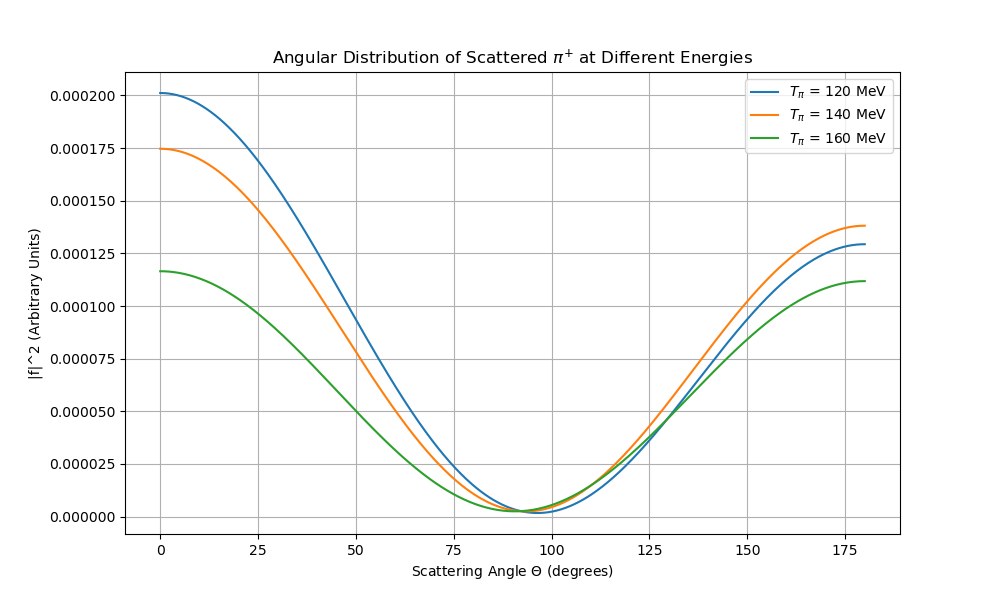
\includegraphics[max width=\textwidth]{angular_distribution.png}
\end{figure}
% Inline Python code in the document
\begin{lstlisting}[language=Python]
import numpy as np
import matplotlib.pyplot as plt

# Define the scattering amplitude function
def scattering_amplitude(p, delta_0, delta_1, theta):
    """
    Calculates the scattering amplitude for given momentum p, phase shifts delta_0 and delta_1, and angle theta.
    """
    term_0 = np.exp(2j * delta_0) - 1
    term_1 = (np.exp(2j * delta_1) - 1) * np.cos(theta)
    return (1 / (2j * p)) * (term_0 + 3 * term_1)

# Calculate the angular distribution |f|^2
def angular_distribution(p, delta_0, delta_1, theta):
    f = scattering_amplitude(p, delta_0, delta_1, theta)
    return np.abs(f)**2

# Energies of interest
energies = [120, 140, 160]  # MeV

# Phase shifts at these energies, interpolated from given values
phase_shifts = {
    120: {'delta_0': np.deg2rad(25), 'delta_1': np.deg2rad(68)},  # Updated based on the plot provided earlier
    140: {'delta_0': np.deg2rad(25), 'delta_1': np.deg2rad(90)},
    160: {'delta_0': np.deg2rad(25), 'delta_1': np.deg2rad(111)}
}

# Pion mass
m_pi = 139.6  # MeV/c^2

# Calculate momentum P_pi for each energy
p_pions = {T: np.sqrt(T**2 + 2*m_pi*T) for T in energies}

# Angular range
theta = np.linspace(0, np.pi, 500)  # From 0 to \pi radians

# Plot the angular distribution
plt.figure(figsize=(10, 6))

for T in energies:
    p = p_pions[T]
    delta_0 = phase_shifts[T]['delta_0']
    delta_1 = phase_shifts[T]['delta_1']
    distribution = angular_distribution(p, delta_0, delta_1, theta)
    # convert the angular distribution by dividing by 
    plt.plot(np.degrees(theta), distribution, label=f'$T_{{\pi}}$ = {T} MeV')

plt.title('Angular Distribution of Scattered $\pi^{+}$ at Different Energies')
plt.xlabel('Scattering Angle $\Theta$ (degrees)')
plt.ylabel('|f|^2 (Arbitrary Units)')
plt.legend()
plt.grid(True)
plt.savefig('angular_distribution.png')

\end{lstlisting}
\subsection{}
(d) What is the mean free path of $140 \mathrm{MeV}$ pions in a liquid hydrogen target, with these "protons"?\\\\
The mean free path is given by:
\begin{equation}
\lambda = \frac{1}{n \sigma}
\end{equation}
where $n$ is the number density of the target, and $\sigma$ is the total cross section. The number density of liquid hydrogen is given by:
\begin{equation}
n = 2 \times \frac{\rho N_A}{M}
\end{equation}
where $\rho$ is the density of the liquid hydrogen, $N_A$ is Avogadro's number, and $M$ is the molar mass of hydrogen. We also multiply by 2 because there are two protons per molecule of liquid hydrogen. The molar mass of hydrogen is given by:
\begin{equation}
M = 2.016 \text{ g/mol}
\end{equation}
The density of liquid hydrogen is given by:
\begin{equation}
\rho = 0.0708 \text{ g/cm}^3
\end{equation}
Avogadro's number is given by:
\begin{equation}
N_A = 6.022 \times 10^{23} \text{ mol}^{-1}
\end{equation}
By inspection of the plot of the total cross section, we can see that the total cross section is approximately $2.6 \text{ mb}$ at $140 \text{ MeV}$. After converting to SI units, I calculate the mean free path:
\begin{equation}
\lambda = 90.93 \text{m}
\end{equation}
% Inline Python code in the document
\begin{lstlisting}[language=Python]
# Constants and given values
rho_kg_m3 = 70.8  # kg/m^3, converted density of liquid hydrogen
M_g_mol = 2.016  # g/mol, molar mass of hydrogen
NA = 6.022e23  # mol^-1, Avogadro's number
sigma_m2 = 2.6e-31  # m^2, converted cross-section

# Calculating number density n
n = 2 * (rho_kg_m3 * NA) / (M_g_mol * 1e-3)  # Convert M from g/mol to kg/mol for consistency in SI units

# Calculating mean free path lambda
lambda_mfp = 1 / (n * sigma_m2)

lambda_mfp
\end{lstlisting}

\begin{center}
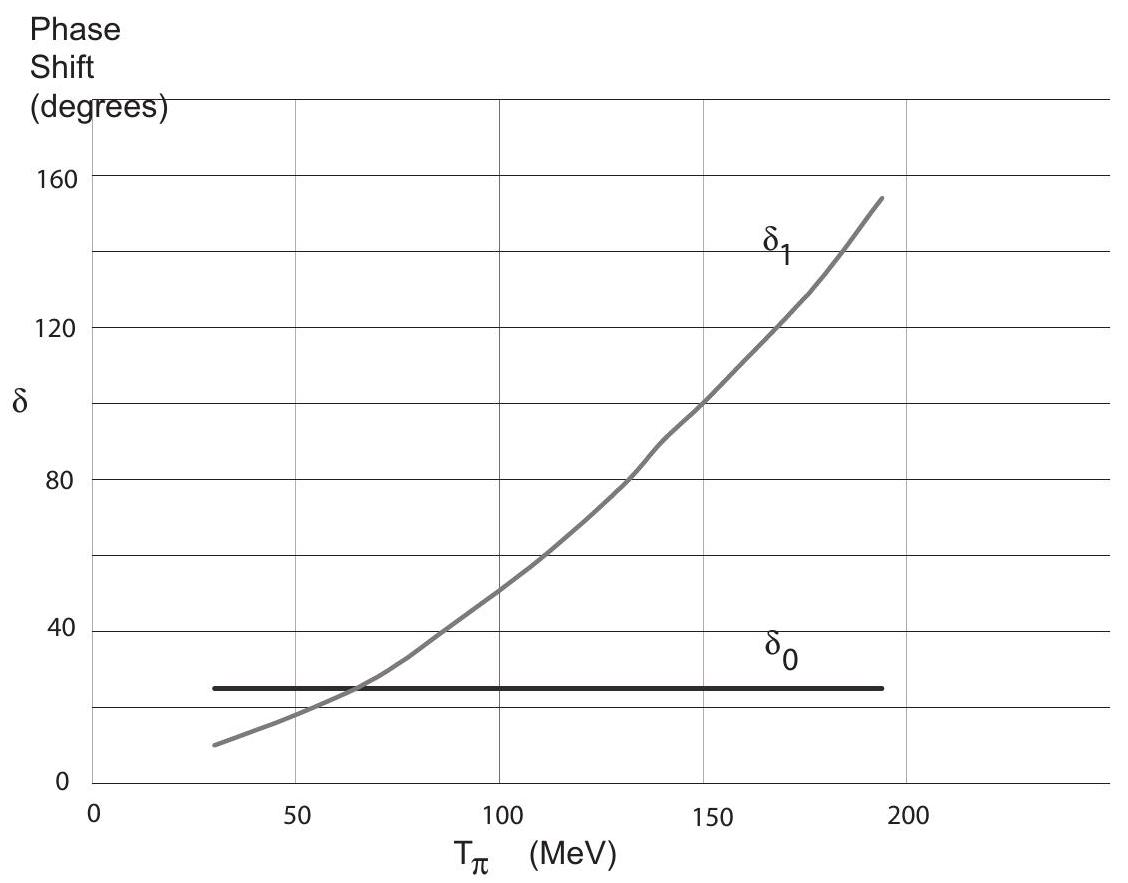
\includegraphics[max width=\textwidth]{2024_03_02_e4ccbaaa87e764c710bfg-3}
\end{center}

Figure 1: Made-up (but motivated by the famous " 33 resonance" in $\pi^{+} p$ scattering) graph of phase shifts $\delta_{0}$ and $\delta_{1}$ for elastic $\pi^{+} p$ scattering (neglecting spin).


\end{document}